\documentclass[openany,12pt,english]{book}
\usepackage[T1]{fontenc}
\usepackage[utf8]{inputenc}
\usepackage{graphicx,color}
\usepackage{bbold}
%\usepackage{fullpage}
\usepackage{geometry}
 \geometry{
 a4paper,
 total={210mm,297mm},
 left=30mm,
 right=25mm,
 top=25mm,
 bottom=25mm,
 }
\usepackage{amsmath}
%\PassOptionsToPackage{hyphens}{url}\usepackage{hyperref}
\usepackage[hyphens]{url}
\usepackage{booktabs}
\usepackage{array}
%\usepackage{multirow}
\usepackage{listings}
%\usepackage[chapter]{algorithm}
\usepackage{algorithmic}
%\usepackage{algpseudocode}
\usepackage{amsfonts}
\usepackage{longtable,enumitem}
\usepackage{tikz}
%\usepackage{indentfirst}
\usepackage{mathrsfs}
\urlstyle{same}
\usepackage{hyperref}
%\usepackage[sorting=none, backend=biber]{biblatex} % load the package
%\addbibresource{biblio.bib} % add a bib-reference file

\usepackage{caption}
%\usepackage[within=none]{newfloat}
\usepackage{rotating}
\usepackage{verbatim}
\usepackage[resetlabels]{multibib} 

\linespread{1.1}
\graphicspath{{./images//}}

\setcounter{secnumdepth}{6}
\setcounter{tocdepth}{6}
\newtheorem{de}{Definizione}[chapter]
\usepackage{amssymb}
\usepackage{verbatim}
\usetikzlibrary{arrows}

\usepackage[english]{babel}
\usepackage{makeidx,multicol}
\usepackage{tabularx}
\newcommand{\RR}{\mathbb{R}}

\newcommand{\NP}{\mbox{\bf NP}}
\newcommand{\PP}{\mbox{\bf P}}
\newcommand{\DT}{\mbox{\bf DTIME}}
\binoppenalty=9999
\relpenalty=9999
\definecolor{gray}{rgb}{0.5,0.5,0.5}
		\lstset{frame=tb,
		  basicstyle=renewcommand\footnotesiz{
\fontsize{10pt}\selectfont}
		  tabsize=2,
		  language=Mathematica,
		  captionpos=b,
		  showstringspaces=false,
		  numbers=left,
		  numberstyle=\tiny\color{gray},
		  columns=fullflexible
		}
		
		\renewcommand{\lstlistingname}{Code}
		\renewcommand{\lstlistlistingname}{List of Codes}
\pagestyle{plain}
\title{Deep Convolutional Neural Network for brain segmentation: Two Pathway architecture} 	
\author{Matteo Causio} %\vspace{0.5cm}}
\date{\textbf{Academic year 2016/2017}}
\begin{document}
	
	\maketitle
	\tableofcontents
	\thispagestyle{empty}
	\newpage
	\chapter{Two-pathways architecture}
	Following the idea of Havaei et. al. in \cite{HAV17} we have implemented a so called \emph{Two-Pathways} Convolutional network made up by a local and a global path. Both two paths get as input the four modality of a patch $33x33$, centered in the pixel that we want to classify, in a slice of a RMI.\\
	The global pathway is made up by a convolutional 2D layer with Rectified Linear activation function and $13x13$ kernels that outputs $160$ feature maps $21x21$ followed by a drop out layer.
	The local pathway is made up by two blocks of convolution and max pooling layer. In the first block we have a convolutional 2D layer with Rectified Linear activation function and $7x7$ kernels plus a max pooling layer with window size $4x4$ followed by a drop out layer; the block outputs $64$ feature maps $24x24$. In the second block we have a convolutional 2D layer with Rectified Linear activation function and $3x3$ kernels plus a max pooling layer with window size $2x2$ followed by a drop out layer; the block outputs $64$ feature maps $21x21$.
	The two path are then merged in a concatenation layer that concatenate the feature maps of both the path and hence outputs  $224$ concatenated feature maps of size $21x21$ that are then fed to the outputs layer.
	The output layer too have a convolutional shape instead of the largely used fully connected layer; this is because of the better performance in test time.
	It is made up by a convolutional layer with kernels $21x21$ followed by a softmax and it outputs a tensor $5x1x1$ expressing the probabilities of each 5 labels for that pixel.
	\begin{figure}[htbp]
		\centering
		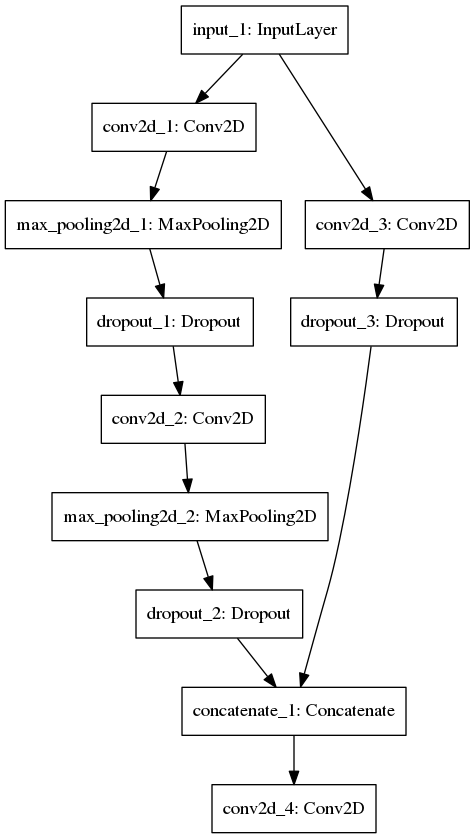
\includegraphics[height=10cm,keepaspectratio]{singleTwoPathModel.png}
		\caption{\protect{Two-pathways model}\label{fig:singleTwoPathModel}}
	\end{figure}

	\chapter{Cascade architecture}
	We have also implemented a cascade architecture model using two convolutional network of the type described above: the output of the first network is concatenated with the input of the second network.
	The first network gets as input the $4$ modalities of a patch $65x65$ around the pixel to classify, then it outputs $5$ feature maps $33x33$ that are concatenated with the $4$ modalities of a smaller patch $33x33$ around the pixel. This $9$ concatenated maps are then fed to the second Two-pathways CNN that outputs a tensor $5x1x1$ expressing the probabilities of each of each $5$ labels. 
	\begin{figure}[htbp]
		\centering
		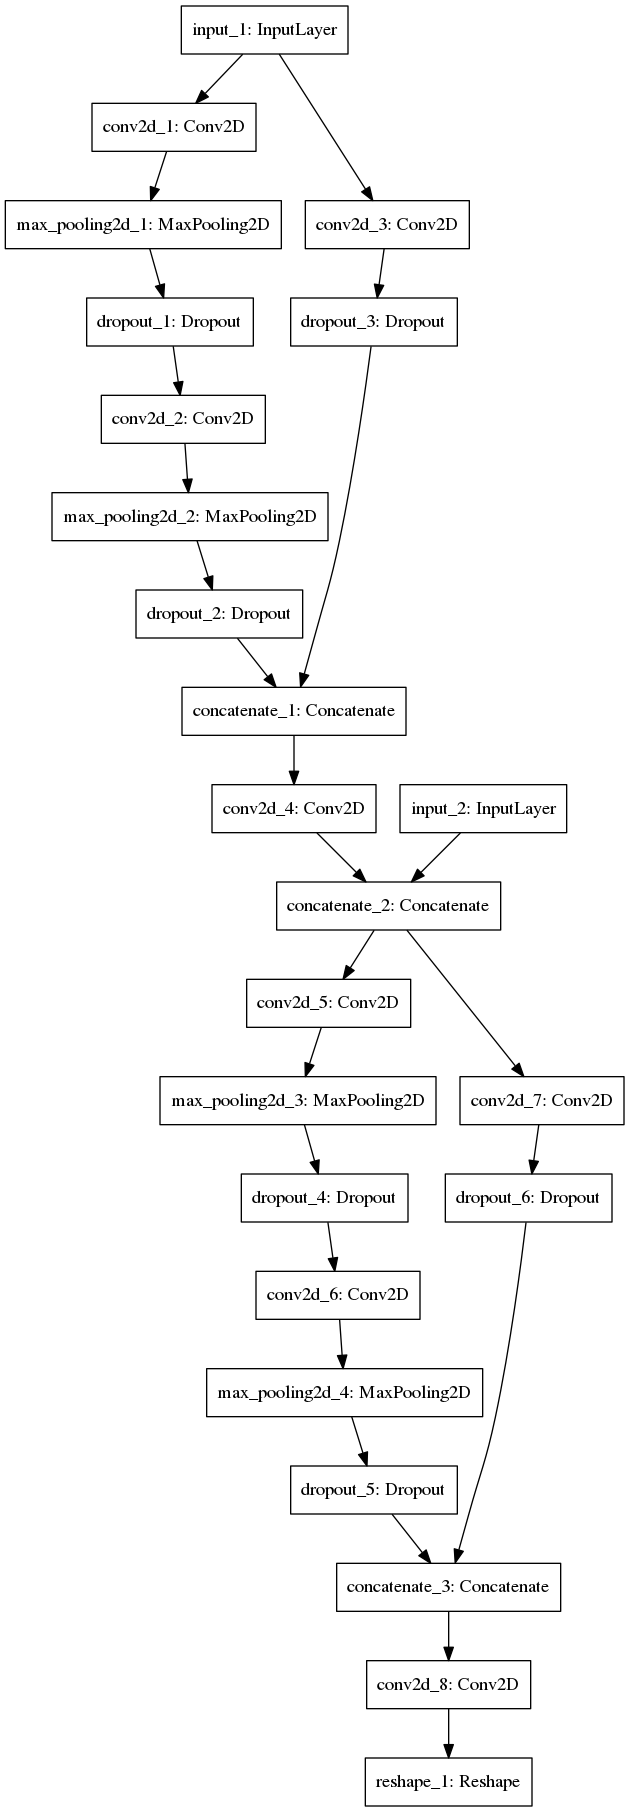
\includegraphics[height=10cm,keepaspectratio]{CascadeModel.png}
		\caption{\protect{Cascade model}\label{fig:CascadeModel}}
	\end{figure}
	 
	Some hyperparameters such as momentum, dropout, learning, decay, l1 and l2 rates have to be determined by cross-validation.
	
	\chapter{Two phase training}
	The training of a single two pathways CNN is divided in two phase to account the unbalanced nature of the data: in fact there are about $98 \%$ pixels classified as healthy, $0.18\%$ as necrosis, $1.1\%$ as edema, $0.12\%$ as non-enhanced and $0.38\%$ as enhanced.
	So in the first phase we train the model using patches with equiprobably labels, in other word for each class we select $\frac{T}{5}$ patches around a pixel labeled with such class; this enable the model to does not be overhelmed by the healthy pixels.
	In the second phase we freeze the parameters of all the layers except the output layer and then we train the parameters of the output layer with truly distributed dataset substrating randomly the $T$ patches from the training set; this permits to calibrate correctly the output probabilities.
	
	\section{Training for the cascade achitecture}
	To train the cascade model we apply the two phase procedure two times; once we have trained the first Two-pathways CNN, we freeze its parameters and then we train the second two pathways CNN.
	To train the first Two-pathways CNN we need $4x33x33$, so we can compare the segmented images and the targets during the training.
	
	\chapter{Implementation}
	We use \emph{python 2.7} and {Keras 2} running on top of \emph{Tensor Flow}.
	We have implemented three classes called \emph{BrainSegDCNN\_2},  \emph{patch\_library} and \emph{image\_preprocessing}
	Follows a description of these classes.
	
	\section{image\_preprocessing}
	The tasks of this class are to load the targets and the $4$ modalities of the RMIs, both in format .mha, and preprocess the latters with normalization and applying \emph{n4 bias field correction} to correct the nonuniformity of the images. Finally it saves to specific folders, in format .png, the targets and the RMIs, compacted into a strip image containing the $4$ modalities.
	The function \emph{save\_patient\_slices} gets as input a list of paths of the RMIs of patients that you want to preprocess; thus to start the preprocessing create such list and execute \emph{save\_patient\_slices} giving as argument the list, the type of preprocessing ('reg' for no preprocessing, 'norm' for normalization, 'n4' for normalization and N4 bias correction) and the boolean \emph{labels} (False if you are preprocessing for testing and there aren't targets to save). Then for each element of the list is initialized a ImagePreProcessing object that takes as arguments the type of preprocessing, an id-number for that specific patient and \emph{labels}; at initialization time the method \emph{read\_scans} loads the RMI of the patient (.mha files) from the given path, concatenates the for modalities of each slice as a strip and then the method \emph{norm\_slices} preprocess them, saves them in a specific folder (\emph{Training\_PNG} for 'reg', \emph{Norm\_PNG} for 'norm', \emph{n4\_PNG} for 'n4') and eventually  the method \emph{save\_labels} saves the targets in \emph{Labels}, naming them with the same name of the relative slice of the patient (\#patient\_\#slice), all as .png files.
	To run this class the following options are available:
	\begin{itemize}
		\item \emph{-path} or \emph{-p} $\mathbf{list(str)}$ (default []) list of the paths of the RMIs to preprocess
		\item \emph{-type} or \emph{-t} $\mathbf{str}$ (default 'reg') type of preprocessing: 'reg' for no preprocessing, 'norm' for normalizing but no bias correction, 'n4' for normilizing and bias correction;
		\item \emph{label} or \emph{-l} $\mathbf{bool}$ (default True) True for training samples with targets, False for test samples without targets.
	\end{itemize}
	
	\section{patch\_library}
	This class is a patches extractor that selects classified pixels from the targets and exctract the relative $33x33$ and, in the (default) case of cascade architecture, the $65x65$ patches around that pixel from each modality of RMIs.
	Setting the arguments $\mathbf{patch\_size=(33,33)}$ and $\mathbf{subpatches\_33=False}$ you fall in the former case.It is useful to create the training set. At initializing time of the class \emph{PatchLibrary}, its method \emph{set\_train\_data} is executed to couple togethere the path of a sample and the relative targets in a list and then saves it in the field \emph{train\_data}. The class takes as arguments a list of paths where are saved the RMIs for training in format .png (created by the preprocessing), the number of patches needed to be selected, the path of the folder containing the labels, the size of the patches (default (65,65)) and the boolean value \emph{subpatches\_33} (default True) to extract the 33x33 subpatches to each patch selected.
	Then executing the PatchLibrary's method \emph{make\_training\_patches} produces a list of 65x65 patches, a list of their 33x33 subpatches centered on the central pixel and a list of the labels for the central pixel of each patches in the default case of cascade architecture;in the other case it produces just a list of 33x33 patches and a list of the label of each central pixel. Setting the argument $\mathbf{balanced\_classes=True}$, \emph{make\_training\_patches} executes the method \emph{find\_balanced\_patches}, otherwise (default case) the method \emph{find\_patches} is executed.
	The method \emph{find\_balanced\_patches} selects $\frac{n}{5}$ pixels for each class, where $n$ is the size of the training set, and extract the relative patches from RMIs; it is necessary for the first phase of the training where the labels have to be equiprobably.
	The method \emph{find\_patches} select randomly $n$ pixels and extract the surrounding patches from RMIs modalities to create the training set needed to train the output layer during the second phase of training, where the labels have the true distribution.

	\section{BrainSegDCNN\_2}
	This is the class designated to create and train the neural network and to make predictions on new data. The network is implemented using \emph{Model} class in Keras.
	Setting the boolean field \emph{cascade\_model} we can create either a single Two-pathways CNN(False) or the cascade model of two of these; during initialization the field \emph{model} is setted using the method \emph{comp\_model}.
	Method \emph{comp\_model} first creates and compiles a single CNN and sets the field \emph{cnn1} to it, then if the field \emph{cascade\_model} is True , the cascade model is created and compiled using cnn1 as first part of the network followed by another single Two-pathways CNN and the field \emph{model} is setted to it, otherwise the field \emph{model} is set to \emph{cnn1}.
	The two phase training of the model is executed by the method \emph{fit\_model} that calls the helper method \emph{freeze\_model} to freeze the weights of the network and \emph{fit\_cnn1} to fit the first Two-pathways CNN; this method can fit either the single and cascade model.. To train the first two path CNN we need to have inputs of shape $4x33x33$, so in \emph{fit\_cnn1} we train a temporary Two-pathways CNN with such input shape and then we set the parameters of the CNN with input $4x65x65$ equal to the weights of the trained CNN with input $4x33x33$.
	The method \emph{show\_segmented\_image} make prediction on new data using the \emph{Model.predict} in Keras and show the segmented image using the library \emph{matplotlib.pyplot}.
	There are also the method \emph{save\_model} and \emph{load\_model} to save and load a model and the values of their weights. 
	To run this class the following options are available:
	\begin{itemize}
		\item \emph{-cascade} or \emph{-c} $\mathbf{bool}$ (default False) for choosing between the single or cascade architecture;
		\item \emph{-train} or \emph{-t} $\mathbf{int}$ (default 1000) to set the number of samples to train the model;
		\item \emph{-samplespath} or \emph{-sp} $\mathbf{str}$ (default 'Training\_PNG') to set the path of the folder containing the samples for training, if needed;
		\item \emph{-labelspath} or \emph{-lp} $\mathbf{str}$ (default 'Labels') to set the path of the folder containing the labels for training, if needed
		\item \emph{-load} or \emph{-l} $\mathbf{str}$ (default 0, no trained model will be loaded) set the name of the already trained model you want to load; if given no training is executed;
		\item \emph{-save} or \emph{-s} $\mathbf{str}$ (default None, the model isn't saved) to set the name you want to save the model after training;
		\item \emph{-test} $\mathbf{str}$ (default None, no segmentation is executed) the path of the folder containing the RMIs that have to be segmented.
	\end{itemize}
	
	
	\clearpage
%\nocite{*}
\bibliographystyle{plain}
\bibliography{bibliography}
\addcontentsline{toc}{chapter}{Bibliografia}


\end{document}